\documentclass[12pt,hidelinks]{article}
\author{Rien Maertens\\
    2\textsuperscript{de} Bachelor Informatica}
    \title{Project Zeepbelbomen}
    \usepackage[utf8]{inputenc}
    \usepackage[dutch]{babel}
    \usepackage{amsthm}
    %\usepackage[a4paper]{geometry}
    %\geometry{tmargin=2.5cm, bmargin=2.5cm, lmargin=2.5cm, rmargin=2.5cm}
    \usepackage{hyperref}
    \usepackage{enumerate}
    \usepackage{mathtools}
    \usepackage{graphicx}
    \usepackage{float}
    \usepackage{tikz}
    \usepackage{pgfplots}
    \usepackage{pgfplotstable}
    \pgfplotsset{compat=1.10}
    \usetikzlibrary{shapes.geometric,arrows,fit,matrix,positioning}
    \tikzset
    {
        tr/.style = {circle, draw=black, align=center, minimum size=1cm}
    }
    \DeclarePairedDelimiter\floor{\lfloor}{\rfloor} 

    \newtheorem{opgave}{Opgave}
    \newtheorem{geval}{Geval}[subsection]
    \newtheorem{stelling}{Stelling}
    \newtheorem{deelresultaat}{Deelresultaat}
    \begin{document}
    \maketitle
    \part{Theoretische Vragen}
    \begin{opgave}
        Geen top in een bladzeepbel heeft een kind in een andere zeepbel.
        \begin{proof}
            Stel we hebben een bladzeepbel $\alpha$ met een top $T$ die een kind $K$ heeft in zeepbel $\beta$. 
            Neem $n$ het aantal zeepbellen dat het pad van zeepbel $\alpha$ naar de wortel bevat. 
            We kunnen de volgende twee gevallen onderscheiden:
            \begin{description}
                \item[Geval 1] Zeepbel $\beta$ bevat een top zonder kinderen en is dus een bladzeepbel.
                    Het pad van de wortel van de boom naar $\beta$ gaat door $\alpha$.
                    Dit pad bevat dus $n+1$ zeepbellen. Dit is tegenstrijdig met het gegeven dat het pad van de wortel naar alle bladzeepbellen evenveel zeepbellen bevat.
                    Het gestelde is dus vals. Het is onmogelijk voor een bladzeepbel om een kind te hebben in een andere zeepbel.
                \item[Geval 2] Zeepbel $\beta$ is geen bladzeepbel, maar bevat wel een pad naar een top zonder kinderen.
                    Deze top is onderdeel van bladzeepbel $\gamma$.
                    Het pad van $\gamma$ naar de wortel van de zeepbelboom bevat $n+k$ zeepbellen, met $k$ het aantal zeepbellen in het pad tussen $\beta$ en $\gamma$.
                    Dit is opnieuw tegenstrijdigi met het gegeven dat het pad van de wortel naar alle bladzeepbellen hetzelfde aantal zeepbellen bevat.
                    Ook in dit geval kan een bladzeepbel geen kinderen in andere zeepbellen hebben.
            \end{description}
        \end{proof}
    \end{opgave}
    \newpage
    \begin{opgave}
        Wat is de maximale diepte van een $k$-zeepbelboom met $n$ sleutels?
        \begin{enumerate}[a.]
            \item Gemeten in zeepbellen. 


                \begingroup 
                \normalfont
                Stel $d_z$ de diepte in zeepbellen van een zeepbelboom. $d_z$ bereikt een maximum wanneer iedere zeepbel maar één top omvat,
                m.a.w. wanneer het pad van de wortel naar een blad evenveel zeepbellen als toppen bevat. 
                De maximale diepte $d_z$ in zeepbellen van een $k$-zeepbelboom met $n$ sleutels is dus gelijk aan de maximale diepte in toppen van een complete binaire boom met $n$ toppen. Dit is dus:
                \begin{equation}
                    d_z \le \floor{\log_2 n}
                \end{equation}
            \endgroup
        \item Gemeten in toppen van de ten gronde liggende binaire boom.


            \begingroup
            \normalfont
            Stel $d_t$ de diepte in toppen van een zeepbelboom. $d_t$ bereikt een maximum wanneer we één lang pad van zeepbellen maken waar elke top van een zeepbel maximum één kind in dezelfde zeepbel bevat. De andere zeepbellen die kinderen zijn van dit lange pad zijn terug zeepbellen met grootte één. Dit ziet er dan als volgt uit:

            \begin{figure}[H]
                \centering


                {
                    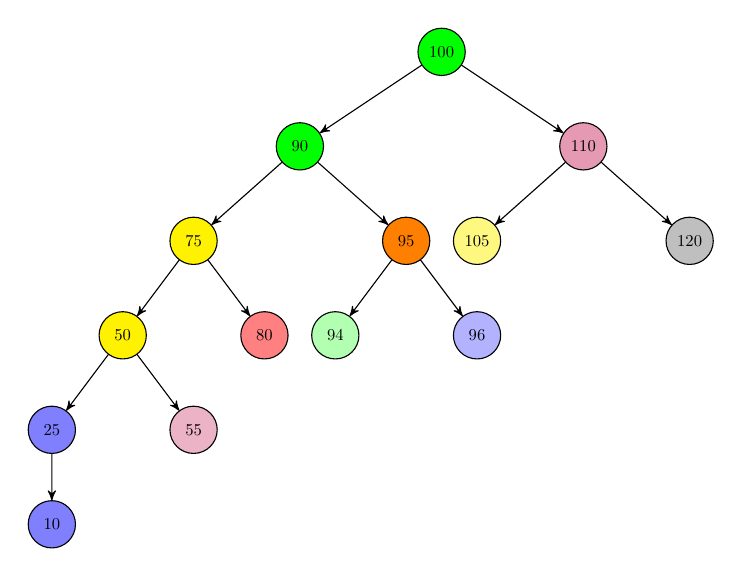
\begin{tikzpicture}[->,>=stealth',
                            level/.style={level distance = 2cm},
                            level 1/.style={sibling distance=6cm},
                            level 2/.style={sibling distance=4.5cm}, 
                            level 3/.style={sibling distance=3cm}, 
                        scale=0.6, transform shape]
                        \node [tr, fill=green] {100}
                        child {
                            node [tr, fill=green] {90} 
                            child {
                                node [tr, fill=yellow] {75} 
                                child {
                                    node [tr, fill=yellow] {50} 
                                    child{
                                        node [tr, fill=blue!50] {25}
                                        child{
                                            node [tr, fill=blue!50] {10}
                                        }
                                    }
                                    child{
                                        node [tr, fill=purple!30] {55}
                                    }
                                }
                                child {
                                    node [tr, fill=red!50] {80} 
                                }
                            }
                            child {
                                node [tr, fill=orange] {95}
                                child{
                                    node [tr, fill=green!30] {94}
                                }
                                child{
                                    node [tr, fill=blue!30] {96}
                                }
                            }
                        }
                        child {
                            node [tr, fill=purple!40] {110}
                            child{
                                node [tr, fill=yellow!50] {105}
                            }
                            child{
                                node [tr, fill=gray!50] {120}
                            }
                        }
                        ;
                    \end{tikzpicture}
                }
            \end{figure}




            Het valt op dat wanneer we een niveau zeepbellen toevoegen, we het dubbele aantal toppen moeten toevoegen van de vorige zeepbelboom met een niveau lager. 
            Voor $n$ het aantal toppen en $z$ het aantal niveaus in zeepbellen geldt: 
            $$n \ge \sum\limits_{i=1}^z k2^{z-1} = k(2^z-1)$$
            We lossen dit op naar $z$: $$z \le \log_2{\left(\dfrac{n+k}{k}\right)}$$
            De maximale diepte $d_t$ van deze zeepbelboom in toppen is gelijk aan het aantal niveaus zeepbellen vermenigvuldigd met het maximale aantal toppen per zeepbel.
            Dus krijgen we dat $d_t=k\cdot z$.
            Wanneer voegen dit alles samen tot één formule:
            \begin{equation}
                d_t \le k \cdot \log_2{\left(\dfrac{n+k}{k}\right)}
                \label{topdiepte}
            \end{equation}
            Waar $d_t$ gelijk is aan de maximale diepte in toppen.
        \endgroup 
\end{enumerate}
    \end{opgave}	
    \begin{opgave}
        Analyse van de verschillende gebalanceerde zeepbelbomen en hun complexiteit.
        \begin{enumerate}[a.]
            \item Voor toevoegen.

                \normalfont
                Het toevoegen van een item aan een gebalanceerde zeepbelboom gebeurt als volgt:

                Eerst wordt het item opgezocht in de zeepbelboom.
                Wanneer het item gevonden werd dan zit het item al in de zeepbelboom en moet er niets gebeuren.
                In dit geval heeft deze bewerking dezelfde tijds- en geheugencomplexiteit als het opzoeken, respectievelijk $O(\log n)$ en $\Theta(1)$ (dit bespreek ik in punt \ref{opzoeken}).

                Als de opzoeking uitkomt op {\tt null} dan zit het toe te voegen item niet in de boom.
                In dit geval wordt er een nieuwe top aangemaakt en bevestigd aan de top die het laatst werd bekeken bij de zoekopdracht.
                De nieuwe top wordt ook toegevoegd aan de zeepbel waarin de ouder zit.
                Indien de zeepbel door deze toevoeging teveel toppen bevat wordt deze gesplitst.
                De manier waarop de zeepbel gesplitst wordt verschilt per implementatie van zeepbelboom:
                \begin{itemize}
                    \item \textbf{Zeepbelboom1} zal zijn zeepbellen splitsen door eerst te kijken of beide kinderen van de wortel in dezelfde zeepbel zitten.
                        Is dit niet het geval dan wordt een rotatie met de bovenste drie zeepbellen uitgevoerd zodat dit wel zo is.
                        Vervolgens wordt de zeepbel gesplitst zodat elk kind van de oude wortel de wortel wordt van een nieuwe zeepbel.
                        De oude wortel wordt daarna toegevoegd aan de zeepbel van zijn ouder, die eventueel opnieuw wordt gesplitst indien deze nu ook overvol zit.
                        Als de oude wortel ook de wortel van de zeebelboom is dan wordt een nieuwe zeepbel aangemaakt.

                        Er wordt enkel binnen dezelfde zeepbel gekeken en omdat de groote van een zeepbel constant is, gebeurt het splitsen van een zeepbel in constante tijd.
                        In het slechtste geval wordt iedere zeepbel vanaf de toegevoegde top tot aan de wortel gesplitst
                        In opgave $2a$ \eqref{topdiepte} hebben we bewezen dat het aantal zeepbellen van de wortel naar een blad maximaal $\floor{\log_2 n}$ is.

                        We kunnen dus concluderen dat voor Zeepbelboom1 met $n$ toppen de toevoegbewerking kost $O(\log n)$ heeft.

                    \item \textbf{Zeepbelboom2} splitst door eerst de zeepbelboom zo goed mogelijk te balanceren. 
                        Hiervoor worden eerst alle toppen in gesorteerde volgorde in een lijst gestoken en vervolgens opgebouwd tot een zo compleet mogelijke binaire boom. 
                        Daarna wordt net zoals Zeepbelboom1 de wortel toegevoegd aan de zeepbel van zijn ouder en vormen de kinderen van deze wortel de wortels van de nieuwe zeepbellen.

                        Net zoals Zeepbelboom1 wordt er enkel binnen dezelfde zeepbel gekeken, echter zal deze zeepbelboom er net iets langer over doen aangezien altijd alle toppen binnen de zeepbel wordt bekeken in plaats van enkel de bovenste drie. 
                        We besluiten dus dat de kost om een een top toe te voegen aan Zeepbelboom2 $O(\log n)$ is voor een boom van $n$ toppen.
                    \item \textbf{Zeepbelboom3} balanceerd net zoals Zeepbelboom2 eerst de toppen in de te grote zeepbel, maar in plaats van enkel de wortel toe te voegen aan de bovenliggende zeepbel worden er meerdere toppen toegevoegd.
                        Hoeveel toppen er toegevoegd worden kan worden aangepast. 
                        Als deze zeepbelboom werd gemaakt met de normale constructor da zullen er zoveel mogelijk toppen worden toegevoegd aan de bovenliggende zeepbel tot deze zijn maximum capactiteit heeft bereikt (maar niet te vol zit).
                        Met een tweede constructor kan er ingesteld worden dat er een maximum staat op het aantal omhoog te duwen toppen en kan dit maximum ook meegegeven worden.
                        Er kan ook ingesteld worden dat er, indien mogelijk, net zoveel toppen aan de bovenliggende zeepbel worden toegevoegd tot deze moet splitsen.

                        Hier geldt hetzelfde als de vorige twee zeepbelbomen: er wordt enkel in dezelfde zeepbel gekeken, wat in constante tijd gebeurt omdat de grootte van de zeepbel constant is.
                        Een splitsing kan een kettingreactie veroorzaken die bovenliggende zeepbellen ook doet splitsen. Maar er zullen maximum $O(\log n)$ van deze splitsingen gebeuren.
                        De toevoegbewerking van Zeepbelboom3 zal dus ook kost $O(\log n)$ hebben voor een boom waar reeds $n$ elementen in zaten
                        opgeslagen.
                \end{itemize}


            \item Voor opzoeken. \label{opzoeken}

                \normalfont
                De drie gebalanceerde zeepbelbomen gebruiken alledrie dezelfde opzoekmethode, dus de complexiteit van deze bewerking is dezelfde.
                Deze methode werkt zoals een normale binaire zoekboom: 

                De wortel wordt vergeleken met het gezochte item. Is het item in de wortel kleiner dan dalen we af naar het rechterkind van de wortel. 
                Is het item in de wortel groter dan dalen we af naar het linkerkind van de wortel.
                Komt de waarde van de wortel overeen met dat van het gezochte item dan hebben we het item gevonden en kunnen we terugkeren uit de functie.
                We blijven op deze manier zoeken tot we het gezochte item gevonden hebben of tot we niet meer verder kunnnen afdalen in de zoekboom (als we null tegenkomen).
                In dit geval zit het gezochte item niet in de zeepbelboom.

                In het slechtste geval zit het item dat wordt gezocht niet in de zeepbelboom en moeten we helemaal tot een blad van de boom afdalen.
                In \eqref{topdiepte} heb ik de maximale diepte in toppen berekend.
                In die formule is $k$ is een constante dus valt die in asymptotische notatie weg.
                We kunnen dus besluiten dat het opzoeken van een element in een gebalanceerde zeepbelboom die $n$ items bevat een kost van $O(\log n)$ heeft.
        \end{enumerate}
    \end{opgave}
    \begin{opgave}
        Bepaal voor semi-splay zeepbelbomen de slechtste-geval complexiteit en de geamortiseerde complexiteit.
        \\ \\ \normalfont
        We introduceren eerst een paar stellingen die we zullen gebruiken in de antwoorden van deze opgave.
        \begin{stelling}Het langste pad van de wortel naar een blad in een semi-splay zeepbelboom is naar boven begrens door $O(\log(n))$ \label{stelling1}
            \begin{proof}Het slechtste geval doet zich voor wanneer alle zeepbellen op één lijn staan.
                De lengte van het pad van de wortel naar de top die zich het verst van de wortel bevind is dan gelijk aan het aantal zeepbellen vermenigvuldigd met de maximale diepte van een zeepbel.
                \\
                \\
                Het aantal zeepbellen $z$ in een zeepbelboom met $n$ toppen en maximaal $k$ toppen per zeepbel is gelijk aan $\floor{n/k}$.
                Aangezien een complete zeepbel altijd gebalanceerd is heeft deze diepte $\log_2{(k)}$. 
                Het langst mogelijke pad van de wortel naar een blad is $\floor{n/k}\cdot\log_2{(k)} = O(n)$ toppen lang.
                \\
                \\
                In asymptotische notatie wordt dit $O(\log(n)$. Dit is precies wat we zochten.
            \end{proof}
        \end{stelling}
        \begin{stelling} Een semi-splay bewerking gebeurt in constante tijd. \label{stelling2}
            \begin{proof}
                Wanneer een splaybewerking wordt uitgevoerd worden alle toppen uit de drie geselecteerde zeepbellen in inorde overlopen en in een lijst gestopt.
                Bij het inorde itereren worden er $3\cdot k$ toppen overlopen, me $k$ de maximale grootte van een zeepbel.
                Vervolgens wordt deze lijst opgedeeld in drie lijsten van lengte $k$ en worden van deze lijsten drie complete gebalanceerde zeepbellen gemaakt.
                Deze drie zeepbellen worden daarna aan elkaar bevestigd en terug in de zeepbelboom geplaatst.
                \\
                \\
                Omdat er altijd binnen de gegeven drie zeepbelle wordt gekeken zal een semisplay bewering altijd $\Theta(k)$ operaties op toppen nodig hebben.
                Maar omdat de $k$ in een zeepbelboom constant is kunnen we zeggen dat een splaybewerking in constante tijd of $\Theta(1)$ tijd verloopt.
            \end{proof}
        \end{stelling}
        \begin{description}
            \item[Slechtste geval]
                \hfill
                \begin{itemize}
                    \item \textbf{Voor toevoegen}\\
                        Het slechtste geval doet zich voor wanneer het toe te voegen item moet toegevoegd worden als kind van de top die zich het verst van de wortel bevind. 
                        Wanneer dit geval is moeten alle toppen over dit pad overlopen worden om de plaats van de toe te voegen top te vinden.
                        Nadat de plaats werd gevonden wordt het nieuwe item toegevoegd, wat een bewerking van constante tijd is.
                        Als de zeepbel waaraan de nieuwe top is toegevoegd vol zit moet deze gebalanceerd worden. Dit gebeurt ook in constante tijd.
                        Vervolgens wordt er vanuit deze zeepbel tot aan de wortel gesplayed.
                        \\
                        \\
                        Uit stelling \ref{stelling1} volgt dat dit langste pad naar boven begrensd wordt door $O(n)$ en uit stelling \ref{stelling2} volgt dat een splaybewerking in constante tijd gebeurt.
                        We kunnen dus besluiten dat een toevoegbewerking op een boom waar reeds $n$ toppen in zitten in het slechtste geval $O(n)$ kost.
                    \item \textbf{Voor opzoeken}\\
                        Een opzoekbewerking is erg gelijkend op een toevoegbewerking. 
                        Het enige verschil is dat bij een zoekbewerking geen top wordt toegevoegd.
                        In het slechtste geval verloopt een opzoekbewerking op een boom van $n$ toppen in $O(n)$ tijd.
                \end{itemize}
            \item[Geamortiseerde complexiteit]
                \hfill
                \begin{stelling}
                    Een reeks van $n > 1$ bewerkingen op een initieel lege semi-splay boom heeft een geamortiseerde complexiteit van $O(n \log n)$, dus is de gemiddelde kost $O(\log n)$ per bewerking.
                    \begin{proof}
                        Ik bewijs dit met behulp van de potentiaalmethode. Voor een lege boom definiëren wij $\Phi(T)=0$.
                        Stel dat $T$ niet leeg is. 
                        Voor een zeepbel $z$ in een semi-splay boom $T$ met een willekeurige $k$-waarde definieren we $A_T(z)$ als het aantal zeepbellen in de deelboom bestaande uit
                        $z$ en al zijn nakomelingen in $T$. Bovendien defineër $L_T(z) = \log(A_T(z))$.
                        De potentiaal van een semi-splay zeepbelboom definiëren wij als:
                        \begin{equation}
                            \Phi(T) = \sum _{z\in T}{L_T(z)}
                        \end{equation}
                        De potentiaal wordt gewijzigd in twee gvallen:
                        \begin{enumerate}[1.]
                            \item Als er een zeepbel wordt toegevoegd (nog zonder de boom te herbalanceren)
                            \item Als tijdens het semi-splayen als gevolg van een toevoeg- of opzoekbewerking er deelbomen vervangen worden
                        \end{enumerate}
                        \begin{deelresultaat}
                            Als een nieuwe zeepbel aan de zeepbelboom $T$ wordt toegevoegd en het resultaat is de boom $T'$ dan geldt $$\Phi(T')-\Phi(T')\le\log(|T'|)$$.
                        \end{deelresultaat}

                        \begin{center}
                            \begin{tabular}{ l | l | p{5cm} }
                                & echte kost & gewijzigde kost \\ \hline
                                top toevoegen & kekeke & $\Phi(U MA)$ \\ \hline
                                top opzoeken & lololo &  $\Phi(U PA)$
                            \end{tabular}
                        \end{center}
                    \end{proof}
                \end{stelling}
        \end{description}
    \end{opgave}



    \part{Implementatie}
    Hieronder volgt er een korte uitleg over de interne structuur en algoritmes die
    ik heb gebruikt voor de implementaties van de zeepbelbomen.
    \section{Binaire boom}
    \subsection{Top}
    Mijn binaire boom bestaat intern uit toppen die hun ouder,  linker en
    rechterkind bijhouden. Om problemen met deze links te vermijden kan de verwijzing
    naar de ouder van een top enkel ingesteld worden wanneer deze top als kind wordt
    aangeduid van een andere top met de methodes {\tt setRightChild()} en {\tt setLeftChild()}. Omdat de wortel van de binaire boom natuurlijk geen
    ouder heeft is er ook een methode die deze verwijzing op {\tt null} zet.
    Een top bevat ook een booleaanse waarde {\tt removed} die functioneert als
    grafsteen. Daarnaast bevat iedere top ook een verwijzing naar de zeepbel waartoe die 
    top behoort.
    \subsection{Zeepbel}
    Om de toppen in groepjes in te delen bestaat de klasse {\tt Zeepbel}. Deze houdt
    enkel zijn wortel bij en het aantal toppen dat deze bezit. Een zeepbel heeft ook de
    methodes {\tt topAdded()} en {\tt topsRemoved()} die de zeepbel waarschuwen wanneer
    er toppen bijgekomen of weggevallen zijn. De methode {\tt topAdded()} heeft ook
    een boolean terug die zegt of de zeepbel te groot is en verkleind moet worden.
    \subsection{Zeepbelboom}
    In de abstracte klasse Zeepbelboom zit de gemeenschappelijke functionaliteit die
    alle zeepbelboom-implementaties delen. Het is enkel de methode {\tt shrinkBubble()}
    die verschilt tussen de verschillende zeepbelbomen. Deze methode zorgt ervoor dat een 
    overvolle zeepbel gesplitst wordt.

    \section{Implementaties zeepbelboom}
    \subsection{Zeepbelboom1}
    De eerste zeepbelboom  lost een overvolle zeepbel op door zo weinig mogelijk
    veranderingen te brengen aan de interne structuur van de boom. Wanneer de wortel van
    de overvolle zeepbel beide kinderen in diezelfde zeepbel heeft dan worden er geen
    wijzigingen aangepast aan de interne structuur: deze twee kinderen vormen de wortels
    voor twee nieuwe zeepbellen en de top wordt toegevoegd aan de bovenliggende zeepbel.
    Als de wortel van de zeepbel maar één kind in dezelfde zeepbel bevat worden de
    eerste drie toppen geroteerd zodat de wortel wel twee kinderen in dezelfde zeepbel
    heeft en er kan gesplitst worden zoals normaal.
    \subsection{BalancingBubbleTree}
    Dit is een superklasse voor alle zeepbelbomen die een zeepbel moeten kunnen balanceren.
    Deze balancering gebeurt door de methode {\tt balanceBubble()}. Dit gebeurt door eerst 
    alle toppen in inorde te overlopen en in een lijst te plaatsen.
    Vervolgens wordt van deze lijst een nieuwe binaire boom opgebouwd door de recursieve
    methode {\tt listToTree()}. Dit balanceren gebeurt in $\Theta (n)$ tijd als we het
    aantal te balanceren toppen als $n$ kiezen. Maar er wordt enkel in één zeepbel
    gebalanceerd en een zeepbel heeft een maximaal aantal toppen, dus werkt deze methode
    in constante tijd.   
    \subsection{Zeepbelboom2}
    Voor de zeepbel gesplitst wordt wordt deze eerst gebalanceerd met de methode
    uit {\tt BalancingBubbleTree}. Daarna wordt op dezelfde manier gesplitst als
    {\tt Zeepbelboom1}.
    \subsection{Zeepbelboom3}
    Deze zeepbel werkt op dezelfde manier als {\tt Zeepbelboom2} echter worden er hier
    zoveel mogelijk toppen aan de bovenliggende zeepbel toegevoegd. Deze zeepbelboom
    kan geconfigureerd worden: er kan gekozen worden om een maximum te zetten op het 
    aantal omhoog te duwen toppen en er kan ingesteld worden dat er geprobeerd wordt
    om net genoeg toppen toe te voegen aan de bovenliggende zeepbel dat die verplicht
    wordt om te splitsen.  
    \section{Functies}
    \subsection{Iterator}
    Een top heeft een methode {\tt traverseInorder()} waarmee er in inorde kan
    geïtereerd worden over zijn kinderen. Aan deze methode worden twee functionele
    interfaces meegegeven: een {\tt consumer} waaraan het volgende element in de iteratie
    wordt aan doorgegeven en een {\tt predicate} die extra restricties kan opleggen over
    welke toppen er geïtereerd mag worden (bijvoorbeeld enkel over de toppen van een
    bepaalde zeepbel.
    Alle iterators maken van deze methode gebruik.
    \subsection{\tt Zeepbelboom.find()}
    De drie basisoperaties: {\tt add()}, {\tt contains()} en {\tt remove()} maken gebruik
    van de methode {\tt find()} om een top op te zoeken. Deze methode werkt door binair
    te zoeken naar een {\tt Top} tot de juiste top gevonden is of tot er {\tt null} werd
    gevonden, waarna de top aan de juiste consumer wordt doorgegeven.
    \subsection{\tt Zeepbelboom.add()}
    Er wordt eerst met {\tt find()} gezocht naar de juiste top, als de top werd gevonden
    dan gebeurt er niets en wordt {\tt false} teruggegeven. Als de top niet werd gevonden
    wordt top toegevoegd op de plaats waar {\tt null} werd tegengekomen en wordt de
    betreffende zeepbel verwittigd van deze toevoeging, waarna er eventueel kan gesplitst
    worden als deze zeepbel overvol is.
    \subsection{\tt Zeepbelboom.contains()}
    Hier wordt enkel met {\tt find()} gezocht en teruggegeven of de top gevonden werd
    of niet.
    \subsection{\tt Zeepbelboom.remove()}
    De te verwijderen top wordt opnieuw gezocht met {\tt find()}. Wanneer de top gevonden
    werd wordt er een grafsteen geplaatst door de {\tt removed} waarde op {\tt true} te
    zetten. Als er een kritiek aantal grafstenen wordt bereikt (standaard 50\%) wordt
    de boom opnieuw opgebouwd zonder de grafstenen.
    \newline \newline
    Ik was begonnen met een implentatie die de toppen echt uit de zeepbelboom verwijdert,
    maar helaas zitten er nog wat bugs in de code en had ik geen tijd meer om deze te
    debuggen. Dus heb ik een werkende implementatie met grafstenen gemaakt.



    \newpage
    \part{Experimenten}
    Nu volgen de resultaten van enkele testen die ik heb uitgevoerd op de zeepbelbomen.
    \section*{Opzet}
    Mijn testresultaten heb ik verkregen door gebruik te maken van de volgende klassen:
    \begin{description}
        \item[\tt TestResult]: klasse die de tijden van de verschillende testen voor een zeepbelboom bijhoud.
            In deze klasse zijn ook een aantal comparators gedefiniëerd zodat kan gesorteerd worden op naam, tijd om iets toe te voegen \ldots
        \item[\tt PerformanceTest]: hier gebeuren de echte testen. 
            Er wordt eerst een lijst van $n$ integers aangemaakt die alle getallen van 1 tot $n$ bevat (willekeurig door elkaar geschud).
            Vervolgens wordt iedere bewerking---toevoegen, opzoeken en verwijderen indien geïmplementeerd--- tien keer na elkaar uitgevoerd op deze lijst van getallen.
            Om de resultaten zo stabiel mogelijk te houden wordt iedere reeks voorafgegaan door eenzelfde bewerking die niet wordt gemeten.
            Ook wordt iedere keer er een nieuwe boom wordt gebruikt de garbagecollection manueel opgeropen.
            \\
            Bij de methode {\tt testAll()} wordt voor iedere zeepbelboom uitgevoerd, voor alle $k$-waarden van 2 tot {\tt maxK} in stappen van 3.
            Het resultaat van deze methode is een lijst van lijsten van testresultaten ({\tt TestResult}).
        \item[\tt PerformanceWriter]: deze klasse gaat de output van de {\tt testAll()}-methode van {\tt PerformanceTest} oproepen en de resultaten uitschrijven naar bestanden per zeepbelboom.
    \end{description}
    Om de meetresultaten zo stabiel mogelijk te houden heb ik het gehele project gecompileerd in een {\tt jar}-bestand met de {\tt PerformanceWriter.main()} als methode die moet uitgevoerd worden.
    Dit gecompileerde bestand heb ik vervolgens een paar uur laten draaien op een linux-machine. 
    Ook heb ik het programma gelimiteerd tot het gebruiken van 50\% van een processorkern.
    \\
    Als argumenten voor de experimenten heb ik als testgrootte 10000000 en als {\tt maxK}  500 meegegeven.
    \section*{Resultaten}
    De resultaten van de meetresultaten door de voorgaande tests kun je in de volgende grafiekjes zien:
    \subsection*{Gebalanceerde zeepbelbomen}
    \begin{figure}[H]\begin{tikzpicture}
            \begin{axis}[title=Add, xlabel=$k$-waarde, ylabel=Tijd (ms), ymax=2000, legend pos=north east, scaled ticks=false, width=13cm, /pgf/number format/.cd, use comma]
                \addplot +[mark=none] table [x=k, y=add]{testresults/Zeepbelboom1_K2_100000.csv};
                \addlegendentry{Zeepbelboom1}
                \addplot +[mark=none] table [x=k, y=add]{testresults/Zeepbelboom2_K2_100000.csv};
                \addlegendentry{Zeepbelboom2}
                \addplot +[mark=none] table [x=k, y=add]{testresults/Zeepbelboom3_K2_100000.csv};
                \addlegendentry{Zeepbelboom3}
            \end{axis}
        \end{tikzpicture}\caption{Add op gebalanceerde zeepbelbomen.}
    \end{figure}
    \begin{figure}[H]\begin{tikzpicture}
            \begin{axis}[title=Contains, xlabel=$k$-waarde, ylabel=Tijd (ms), ymax=2000, legend pos=north east, scaled ticks=false, width=13cm, /pgf/number format/.cd, use comma]
                \addplot +[mark=none] table [x=k, y=contains]{testresults/Zeepbelboom1_K2_100000.csv};
                \addlegendentry{Zeepbelboom1}
                \addplot +[mark=none] table [x=k, y=contains]{testresults/Zeepbelboom2_K2_100000.csv};
                \addlegendentry{Zeepbelboom2}
                \addplot +[mark=none] table [x=k, y=contains]{testresults/Zeepbelboom3_K2_100000.csv};
                \addlegendentry{Zeepbelboom3}
            \end{axis}
        \end{tikzpicture}
        \caption{Contains op gebalanceerde zeepbelbomen.}
    \end{figure}
    \begin{figure}[H]\begin{tikzpicture}
            \begin{axis}[title=Remove, xlabel=$k$-waarde, ylabel=Tijd (ms), ymax=2000, legend pos=north east, scaled ticks=false, width=13cm, /pgf/number format/.cd, use comma]
                \addplot +[mark=none] table [x=k, y=remove]{testresults/Zeepbelboom1_K2_100000.csv};
                \addlegendentry{Zeepbelboom1}
                \addplot +[mark=none] table [x=k, y=remove]{testresults/Zeepbelboom2_K2_100000.csv};
                \addlegendentry{Zeepbelboom2}
                \addplot +[mark=none] table [x=k, y=remove]{testresults/Zeepbelboom3_K2_100000.csv};
                \addlegendentry{Zeepbelboom3}
            \end{axis}
        \end{tikzpicture}\caption{Remove op gebalanceerde zeepbelbomen.}
    \end{figure}

    \subsection*{Zeepbelboom3}
    \begin{figure}[H]\begin{tikzpicture}
            \begin{axis}[title=Zeepbelboom3, xlabel=$k$-waarde, ylabel=Tijd (ms), ymax=1600, legend pos=north east, scaled ticks=false, width=13cm, /pgf/number format/.cd, use comma]
                \addplot +[mark=none] table [x=k, y=add]{testresults/Zeepbelboom3_K2_parentOverflow_100000.csv};
                \addlegendentry{PO}
                \addplot +[mark=none] table [x=k, y=add]{testresults/Zeepbelboom3_K2_maxPushUp5_100000.csv};
                \addlegendentry{max5}
                \addplot +[mark=none] table [x=k, y=add]{testresults/Zeepbelboom3_K2_maxPushUp5_parentOverflow_100000.csv};
                \addlegendentry{max5 PO}
            \end{axis}
        \end{tikzpicture}
        \caption{De verschillende configuraties van Zeepbelboom3.}
    \end{figure}
    \section*{Semi-splay zeepbelbomen}
    \begin{figure}[H]\begin{tikzpicture}
            \begin{axis}[title=Semi-splay zeepbelboom, xlabel=$k$-waarde, ylabel=Tijd (ms), legend pos=north east, scaled ticks=false, width=13cm, /pgf/number format/.cd, use comma]
                \addplot +[mark=none] table [x=k, y=add]{testresults/Zeepbelboom4_K2_100000.csv};
                \addlegendentry{add}
                \addplot +[mark=none] table [x=k, y=contains]{testresults/Zeepbelboom4_K2_100000.csv};
                \addlegendentry{contains}
            \end{axis}
        \end{tikzpicture}
        \caption{Semi-splay zeepbelboom}
    \end{figure}

    \section*{Besluit}

    \end{document}
